\chapter{Results}
\label{ch:results}
The preprocessed dataset, contained in the "cleaneddataset.csv" file, was taken from the Kaggle heart disease dataset and used to assess the performance of the Support Vector Machine (SVM) and Random Forest models. There are 302 samples in this collection, and each sample has 14 variables, including clinical characteristics that are used to identify heart disease.
\\
Key performance indicators like as F1 Score, Accuracy, Precision, and Recall were used to evaluate the models. These measurements provide insight into how well the models categorize patients into those with and without cardiac disease. 
\\

\\
\section{Performance Comparison of SVM and Random Forest Models}


The performance of two machine learning models, Random Forest and SVM, was evaluated and compared in this study. The models were trained and tested on a specific dataset, and their performance metrics are presented in Tables 4.1 and 4.2.
\\
\begin{table}[h]
\centering
\caption{SVM Model Performance Metrics}
\begin{tabular}{|c|c|c|}
\hline
Metric & Training Value & Testing Value \\
\hline
Accuracy & 0.863 & 0.770 \\
\hline
Precision & 0.854 & 0.727\\
\hline
Recall & 0.911 & 0.827 \\
\hline
F1 Score & 0.882 & 0.774 \\
\hline
\end{tabular}
\end{table}

\\
Table 4.1 displays the performance characteristics of the SVM model. The model achieved an accuracy of 0.863 during training and 0.770 during testing. The precision of the SVM model was 0.854 during training and 0.727 during testing. The recall of the model was 0.911 during training and 0.827 during testing. The F1 score of the SVM model was 0.882 during training and 0.774 during testing.
\\
\begin{table}[h]
\centering
\caption{Random Forest Model Performance Metrics}
\begin{tabular}{|c|c|c|}
\hline
Metric & Training Value & Testing Value \\
\hline
Accuracy & 0.913 & 0.803 \\
\hline
Precision & 0.895 & 0.742 \\
\hline
Recall & 0.955 & 0.896 \\
\hline
F1 Score & 0.925 & 0.812 \\
\hline
\end{tabular}
\end{table}


\\
Table 4.2 presents the performance metrics of the Random Forest model. The model achieved an accuracy of 0.913 during training and 0.803 during testing. The precision of the Random Forest model was 0.895 during training and 0.742 during testing. The recall of the model was 0.955 during training and 0.896 during testing. The F1 score of the Random Forest model was 0.925 during training and 0.812 during testing.
\\
\newpage

\section{Evaluation of Heart Disease Classification: Training and Testing Confusion Matrices}


\begin{figure}[H]
    \centering
    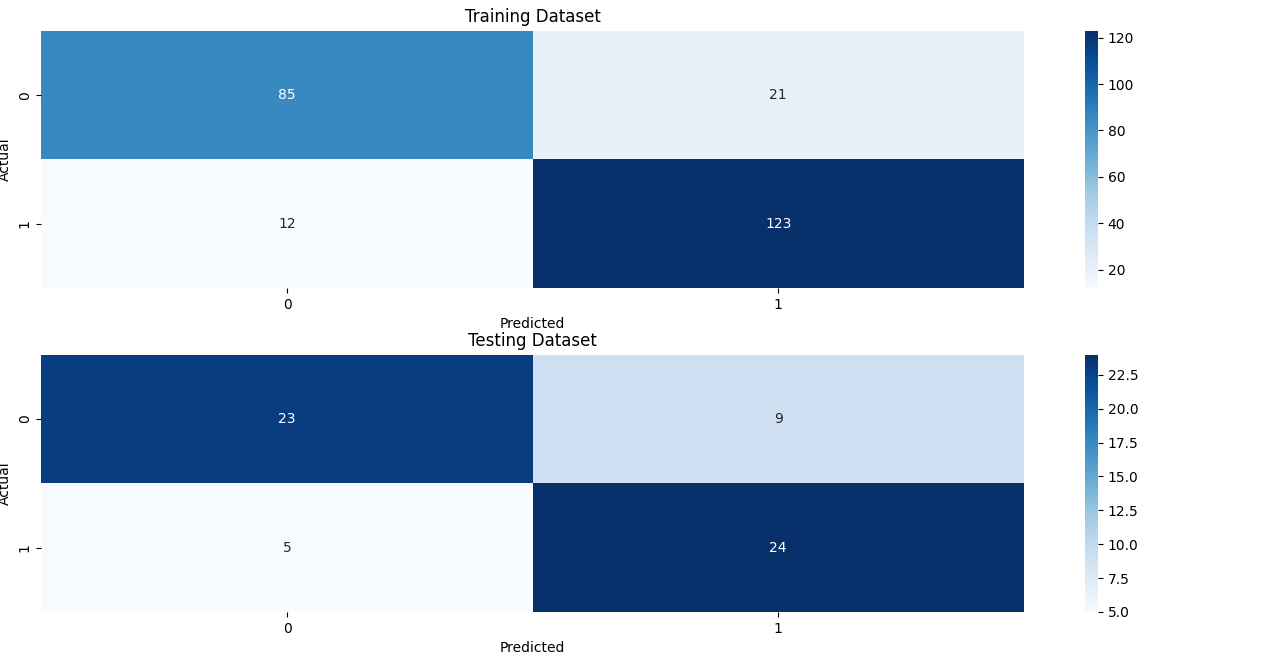
\includegraphics[width=1.0\textwidth]{figures/svm_CM.png}
    \caption{SVM Training and Testing Confusion Matrix}
    \label{fig:svm_cm}
\end{figure}
The SVM model achieved a training accuracy of 86.31 and a testing accuracy of 77.05. In the training set, it correctly classified 85 cases of no heart disease and 123 cases of heart disease, with 21 false positives and 12 false negatives. In the testing set, it correctly classified 23 cases of no heart disease and 24 cases of heart disease, with 9 false positives and 5 false negatives.

\begin{figure}[H]
    \centering
    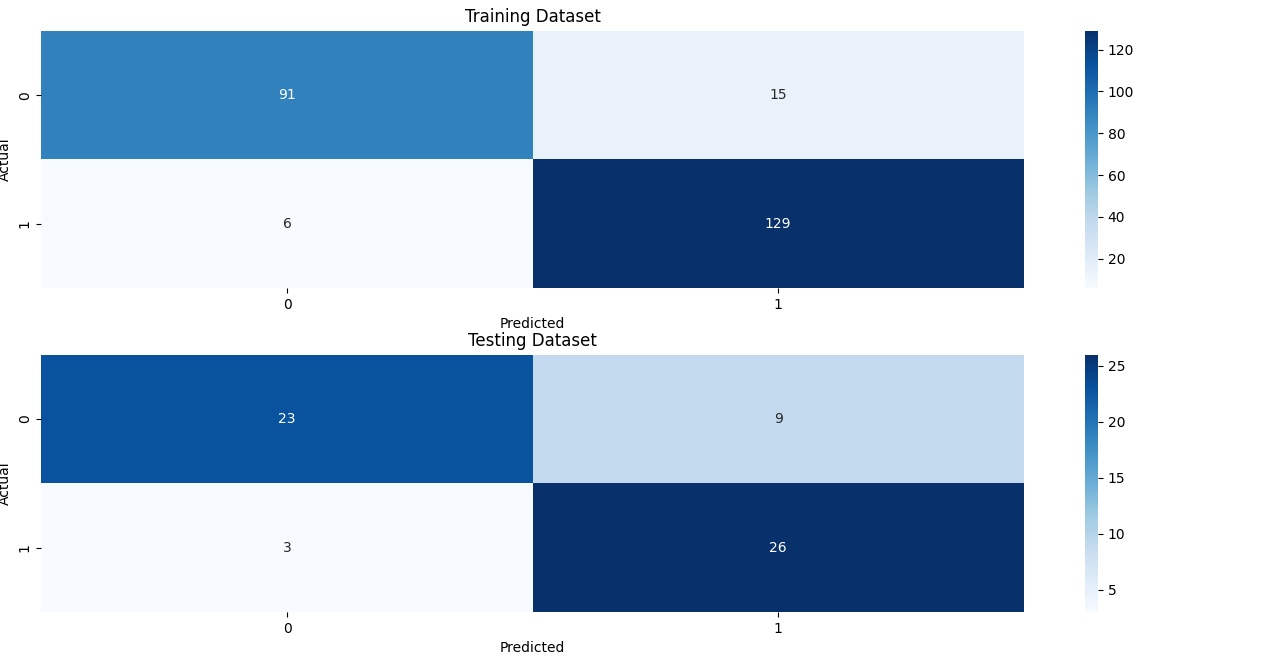
\includegraphics[width=1.0\textwidth]{figures/RF_CM.png}
    \caption{RF Training and Testing Confusion Matrix}
    \label{fig:rf_cm}
\end{figure}
The Random Forest model achieved a training accuracy of 91.29 and a testing accuracy of 80.33. In the training set, it correctly classified 91 cases of no heart disease and 129 cases of heart disease, with 15 false positives and 6 false negatives. In the testing set, it correctly classified 23 cases of no heart disease and 26 cases of heart disease, with 9 false positives and 3 false negatives.

\section{Results Summary}

There was a notable distinction in the SVM and Random Forest models' performance based on the information presented in the tables and confusion matrices. For both the training and testing datasets, the Random Forest model performed better than the SVM model in terms of precision, recall, precision, and F1 score.
